\documentclass{FR16} 

\begin{document}


\maketitle

\tableofcontents
\newpage

\section{Introduction}

\subsection{Overview}
Accelerometer is a mechanical pendulous accelerometer, which serves to sense the linear motion information of the carrier. As the core structural device of an inertial navigation system, its degree of precision and quality of property greatly determine the precision and property of the inertial navigation system. The system is widely applied to missiles, satellites, rockets, and other aircraft and plays a significant part in guaranteeing the vehicle attitude being stable and the target being accurate.
Under the influences of time and external environment, factors like material, process, and manufacturing would trigger the internal stress release and redistribution, lead into drift of
key parameters (zero bias and scale factor), and finally cause
ubiquitous problems during the use of the accelerometer, such
as poor long-term repeatability, short periodical calibration,
complex operation, and maintenance.

Therefore, the precision and long-term repeatability requirements of the inertial navigation system should be handled with due care. Failure to do so may seriously affect  the production delivery schedule of the inertial navigation system

\subsection{Long-term repeatability}
Long-term repetability is  one of the most important parameters that determine the reliability and overall measurement accuracy of a  sensor. Long-term stability in sensors is defined by the maximum acceptable change in zero and span values during the course of the calibration interval of the sensor. In short, for a sensor to be considered stable, it should maintain a very low drift in its measurements over the calibration interval.

Thus, Obtaining long-term stability parameter is not just a requisite but indispensable for precision systems. 


\subsection{Need to measure long-term repeatability}
Improving the long-term stability of the accelerometer involves understanding the various drift causing elements and making corrections or adjustments to these processes:
\begin{enumerate}
    \item \textbf{Internal factors:}The internal factors include the material, structure, component, circuit, manufacturing, and  specifically, accelerometer model coefficients.
     \begin{itemize}
         \item \textbf{Instablility}The Instability when quantified shall give us insights on the following parameters: Residual stress of the internal structural material, magnetization and demagnetization effects of
         the torquer, internal stress by processing and assembly of the mechanical structure and circuit stability
     \end{itemize}
    
    
    \item \textbf{Environmental factors:}The accelerometer is composed of a header and a servo circuit, which is a balanced and regulatory system for force feedback. Its header consists of a pendulous component, a torquer, a soft magnet, a differential capacitance sensor, and other parts. It is an integrated complex of different materials like quartz, magnet, coil, epoxy glue, and electronic circuit. Before the assembly of the accelerometer, all its inner components go through stabilization treatment. However, after the overall manufacture and assembly of the product, the parameters still drift in storage condition under the influence of time and environment. There are mainly two reasons:
        \begin{itemize}
            \item \textbf{Temperature Stress:} Temperature stress is produced by the constraint of material
temperature deformation. It mainly happens inside the core,
where temperature is obviously changed because Joule heat is
generated by the torque coil in the electrifying state (it is more the case for wide-range accelerometers). It is mainly produced by different thermal expansion coefficients of pendulous components like torque coil, epoxy glue, and quartz. In particular, the high-polymer epoxy glue would cause glassy and rubber state transition at a certain temperature, and its mechanical properties such as elastic modulus would change greatly, which could produce greater temperature stress under conditions of temperature change.
            \item \textbf{Residual Stress:}Residual stress is what still remains in the bodies for
self-equilibrium after the external force is eliminated or the
nonuniform temperature field is applied. It is an internal stress produced by the product machining, assembly, and other reasons, and its changes are mainly reflected in the associative
part because, in the process of component assembly, residual
stresses inside components go through release or redistribution under different boundary constraint conditions. For the
accelerometer, residual stress is mainly produced in the pre-loading ring welded joint or the torque coil joint under the
impact of epoxy glue solidification.
From the overall point of view, the key parts of internal stress
release are the adhesive torque coil and the preloading ring
welded joints. Thus, the analysis is necessary to find out what
kind of stress is conducive to the product stability.
    \end{itemize}
     
     
     
\end{enumerate}



\subsection{Quantifying long-term repeatability}
Quantification of the long-term stability parameter requires an automated DAQ capable of acquiring both the acceleration and temperature from all the sensors with storing onto a server with post-analysis capability.

\subsection{Advantage gained through an automated DAQ}
By automating this data-acquiring protocol, the advantages gained are as follows:
\begin{itemize}
    \item \textbf{Reduction in wastage:}As every entry composes of seven to eight digits of accuracy, it  is prone to human errors during manual entry. This may result in dispensing away complete accelerometer system. Such wastage of resources could be avoided by a automated stand-alone DAQ . 
   
    \item \textbf{Increased throughput or productivity:}By automating this testing procedure/protocol, it would become possible to engage a precious human resource elsewhere.
    
    \item \textbf{Reduction in time taken for testing :} Not only it is possible to follow elaborate test sequences but also it can be done without interruption, thus reducing the overall time taken for testing. The users can benefit from the fact that the automation helps the testing to take place without any interruption or input from the user.
   
\end{itemize}


Thus, a well placed data acquisition clubbed with testing automation allows for elaborate test sequences without interruption leading to reduction in time.

Not only we aim to automate the protocols that lead to data acquisition, but also wish to assist them in post data acquisition. To this end, we shall be automating the myriad calculations that needs to be performed to obtain the many system derived performance parameters and many reports that needs to be generated.

The next section deals with the scope of this project. The goals that the project needs to accomplish are described in detail in the following section.


\newpage
\section{scope/Project goal and objectives}
\subsection{Requisite:}
Measure the acceleration and the temperature from the  sensor to an accuracy of 1\textmu g over an extended duration typically ranging over few weeks to a month as specified by the user. All the information needs to be logged with desired 1\textmu g accuracy as a stand alone system.  The final report generation hence forth is also automated with the desired graphical representation. 

This stand alone system should be capable of acquiring, logging and analysis to obtain scale-factor (SF) and stability factors to reflect 1\textmu g inaccuracies. 


The work plan for fulfilling the scope of this project is described in the next chapter.      
\newpage


\section{Work plan/Plan of action}
\subsection{Project Output}
The plan of action has been designed keeping the ruggedness, sustainability and user friendliness at the forefront. Automation is planned in such a way that the user can treat it as a turn key system. Furthermore, aspects like  IoT and remote data access should also be incorporated. This automation would obviate weeks of manual work equivalent to few weeks to a month of data acquisition

\subsection{Division of work}
our work plan is fourfold and execution of it shall proceed in four phases:
\begin{enumerate}
     \item  \textbf{Phase 1:} Programming SOC FPGA 
    \item  \textbf{Phase 2:} Designing an IOT system
    \item \textbf{Phase 3:}  Designing Mechanical fixture
    \item \textbf{Phase 4:} A Desktop application to access and analyse data.
\end{enumerate}
  \begin{figure}[H]
    \begin{subfigure}{\textwidth}
    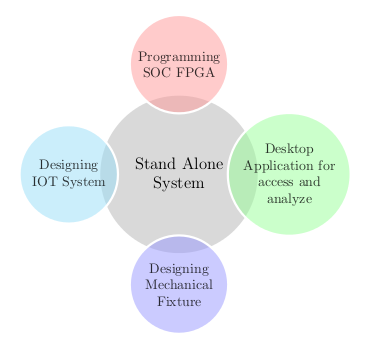
\includegraphics[scale=1]{smart-bubbles.png} 
    \label{fig:DJp1}
    \end{subfigure}
%    \begin{subfigure}{0.5\textwidth}
%    \includegraphics[width=1.0\linewidth, height=5cm]{images/DJ_profile2.png}
%    \label{fig:DJp2}
%    \end{subfigure}
 
 %\caption{Pictorial depiction of our Work-flow}

\label{fig6}
\end{figure}

\subsection{Salient Features}
\begin{itemize}
    \item Precision reflecting 1\textmu g inaccuracies
    \item Nano-second switching
    \item 85dB filter rejection of 50Hz and 60Hz
    \item Channel scan data rate of \sim 10kSPS per channel (100\textmu s settling)
    \item An IOT enabled data-acquisition
    \item Additional Desktop application 
    \item precision reflecting 1\textmu g inaccuracies
    

\end{itemize}


Each of these Phases are described briefly  as a separate section below.
\newpage
\section{Phase1 : Programming SOC FPGA}

The first phase and the most prominent step in the implementation of this stand-alone system shall be programming System on Chip (SOC) Field Programmable Gate Array (FPGA). Moreover, Care is taken throughout
the report that the idea is conveyed more through the medium of images rather than writing few lengthy paragraphs.

\subsection{Phase1 goal and objectives}

\subsubsection{Hardware front}
The objective of this phase is to design and install a SOC FPGA system which can acquire acceleration from 8 different channels. Very accurate data needs to be acquired (upto seven and half decimal accuracy), as these sensors are  utilized in the navigation systems. 

Although FPGA technology might at first seem to not be suitable for the implementation of analog components such as a DAC, their architectures turn out to be very suitable for sigma-delta converters which are primarily digital. Having the flexibility to incorporate DACs into FPGA designs allow for higher levels of integration, reducing cost, board area and possibly power consumption.

An arm based processor with decent RAM like 8GB RAM shall be required and shall act as the master  for all the acquisition.



  \begin{figure}[H]
 
    \begin{subfigure}{\textwidth}
    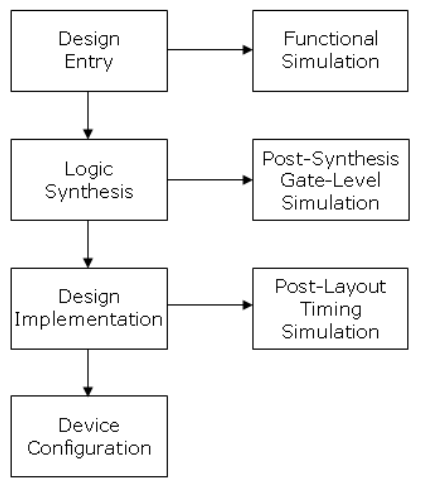
\includegraphics[scale=0.8]{fpga_designflow.png} 
    \label{fig:DJp1}
    \end{subfigure}
%    \begin{subfigure}{0.5\textwidth}
%    \includegraphics[width=1.0\linewidth, height=5cm]{images/DJ_profile2.png}
%    \label{fig:DJp2}
%    \end{subfigure}
 
 \caption{Standard FPGA design flow}
\label{fig6}
\end{figure}








\subsubsection{Software front on programming for sigma-delta}
On the software front the desired goal is achieved by the following design flow and methodologies as described below:
From the technical standpoint, this phase shall be executed in the following manner and may be considered as a three-fold path:

  \begin{figure}[H]
 
    \begin{subfigure}{\textwidth}
    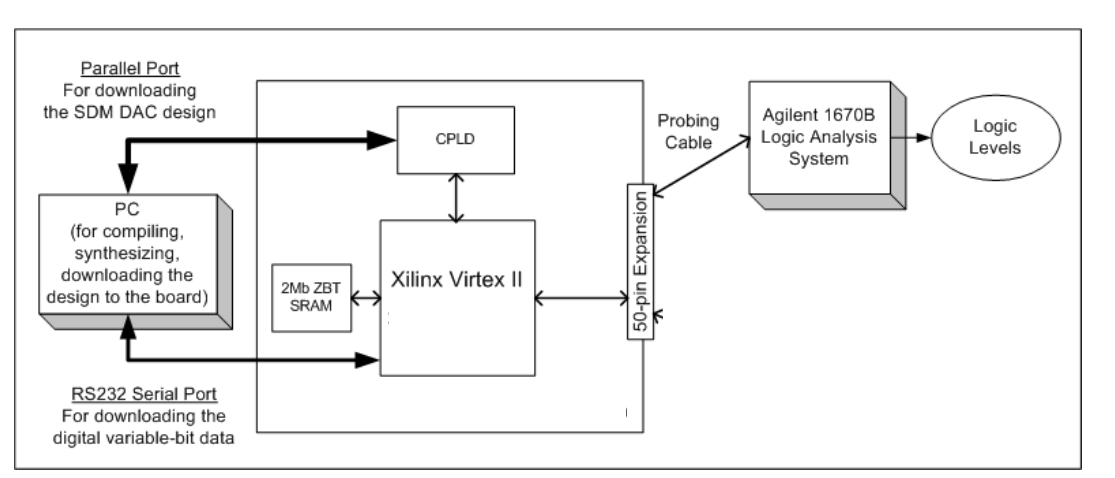
\includegraphics[scale=0.5]{Pictorial_dipiction.png} 
    \label{fig:DJp1}
    \end{subfigure}
%    \begin{subfigure}{0.5\textwidth}
%    \includegraphics[width=1.0\linewidth, height=5cm]{images/DJ_profile2.png}
%    \label{fig:DJp2}
%    \end{subfigure}
 
 \caption{Design Flow}
\label{fig6}
\end{figure}
    


\begin{enumerate}
    \item \textbf{Verilog} The FPGA shall be coded in verilog to obtain the Delta-Sigma Modulator. It consists of a difference amplifier that sums in the feedback of the output, an integrator which acts as noise shaping in that it removes noise in the lower frequencies, a 1 bit comparator, and a switch which effectively feeds back an inverted form of the results of the last sample. Due to the feedback path the digital output represents the difference in signal from sample to sample. 
    \item \textbf{Interpolation} The architecture of the 64 $\times$ / 128 $\times$ /192 $\times$ interpolation filter is shown in Figure 2. It is a multi-stage filter. The
first two half-band filters are non-configurable. They
increase the sampling rate of the signal by four times. The
last stage is a programmable sinc filter to provide variant
interpolation ratios.

     
      \begin{figure}[H]
 
    \begin{subfigure}{\textwidth}
    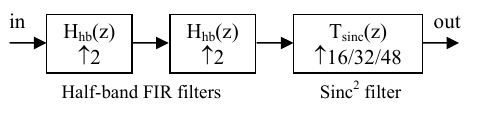
\includegraphics[scale=1]{Interpolation_filter.png} 
    \label{fig:DJp1}
    \end{subfigure}
%    \begin{subfigure}{0.5\textwidth}
%    \includegraphics[width=1.0\linewidth, height=5cm]{images/DJ_profile2.png}
%    \label{fig:DJp2}
%    \end{subfigure}
 
 \caption{Interpolation filter}
\label{fig6}
\end{figure}
    
 
 
 
   \begin{figure}[H]
 
    \begin{subfigure}{\textwidth}
    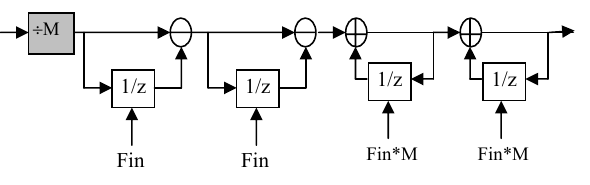
\includegraphics[scale=1]{Blockdiagram_sinc2.png} 
    \label{fig:DJp1}
    \end{subfigure}
%    \begin{subfigure}{0.5\textwidth}
%    \includegraphics[width=1.0\linewidth, height=5cm]{images/DJ_profile2.png}
%    \label{fig:DJp2}
%    \end{subfigure}
 
 \caption{Block diagram of sinc$^{2}$ filter where F$_{in}$ is the sampling input frequency and  M of the sinc filter can be set as 16, 32 and 48 for the overall interpolation ratios of 64$\times$, 128$\times$  and 192$\times$ respectively.}
\label{fig6}
\end{figure}
    
 
   \begin{figure}[H]
 
    \begin{subfigure}{\textwidth}
    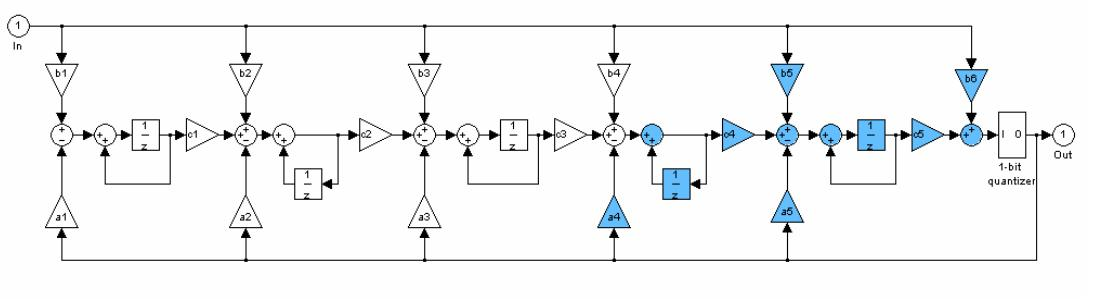
\includegraphics[scale=0.55]{Architechture_5_3.jpeg} 
    \label{fig:DJp1}
    \end{subfigure}
%    \begin{subfigure}{0.5\textwidth}
%    \includegraphics[width=1.0\linewidth, height=5cm]{images/DJ_profile2.png}
%    \label{fig:DJp2}
%    \end{subfigure}
 
 \caption{Architecture of the re-configurable 5th/3rd order sigma-delta modulator}
\label{fig6}
\end{figure}
    
 \item \textbf{Noise shaping}The Delta-Sigma ADC utilizes this noise reduction technique but then goes one step further utilizing a technique known as noise shaping. As the Delta-Sigma modulator uses an integration stage or two, it has a natural traffic shaping effect where the noise at the low end is reduced at the expense of the upper end of the spectrum. Once again we are not really removing the noise outright, but it is reducing the noise in amplitude in the area of interest near our signal. 
    .
 \item \textbf{Typical Pseudo code}A typical pseudo code for the achieving the above mentioned blocks shall be as follows:

   \begin{figure}[H]
 
    \begin{subfigure}{\textwidth}
    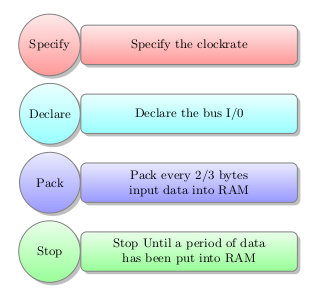
\includegraphics[scale=1]{analysis.png} 
    \label{fig:DJp1}
    \end{subfigure}
%    \begin{subfigure}{0.5\textwidth}
%    \includegraphics[width=1.0\linewidth, height=5cm]{images/DJ_profile2.png}
%    \label{fig:DJp2}
%    \end{subfigure}
 
% \caption{Static code implementation}
\label{fig6}
\end{figure}



   \begin{figure}[H]
 
    \begin{subfigure}{\textwidth}
    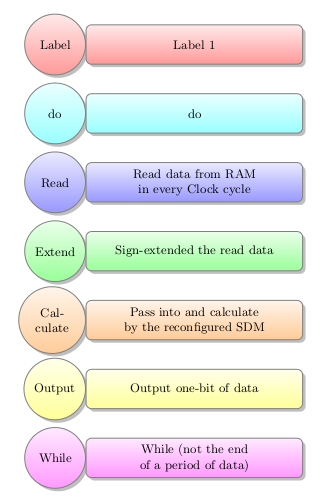
\includegraphics[scale=1]{analysis1.png} 
    \label{fig:DJp1}
    \end{subfigure}
%    \begin{subfigure}{0.5\textwidth}
%    \includegraphics[width=1.0\linewidth, height=5cm]{images/DJ_profile2.png}
%    \label{fig:DJp2}
%    \end{subfigure}
 
% \caption{Pseudo code of the implementation}
\label{fig6}
\end{figure}


\end{enumerate}

\newpage

\section{Phase 2 : Designing an IOT system}
This attempt during this phase shall be to measure and store any kind of electrical and non-electrical signals in embedded web server and be able to control the devices remotely.

\subsection{Introduction to RTOS}
To  heighten the  reliance on technology to execute crucial tasks implementation has led to the usage of high-performance real-time operating systems(RTOS) in this project. 

A real-time operating system (RTOS) is an operating system that works in real time, with deterministic constraints that require efficient time usage and power to process incoming data and relay the expected results without any unknown or unexpected delays. RTOS software is time dependent, meaning that it should process input and offer output within a short predetermined deterministic period. However the key to an RTOS, and the most important demand of RTOS software is that a request and response for data is guaranteed to occur. If a Windows OS has request and response calls that are fast 90\% of the time, yet the remaining 10\% of the time an input/output request takes too long, then the real-time application is not performing correctly. Thus an RTOS is not meant to be only fast, it is more importantly meant to be dependable

\subsection{Client-Server Architecture}
A web server is a system which hosts websites and provides services for any requesting clients. The general
purpose web server composes of an operating system, web pages or web applications and a huge amount of memory
and sometimes a special hardware. The following figure Shows the typical client-server architecture.


A Client can
access the industry’s web server through internet and LAN router. Digitally acquired data are stored in web server’s
data base. Whenever the client wants to access data, it sends the request to server; this request is taken by the router,
which is connected to the internet. The web processes the request made and finally connects to the desired web
server, access the requested data and sends the data to the client.
A web server is a system which hosts websites and provides services for any requesting clients. The general purpose web server composes of an operating system, web pages or web applications and a huge amount of memory and sometimes a special hardware. The following figure shows the typical client-server architecture. 

  \begin{figure}[H]
 
    \begin{subfigure}{\textwidth}
    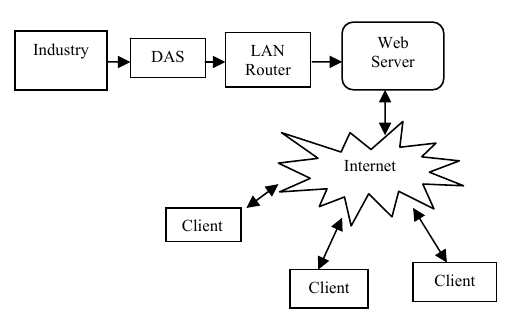
\includegraphics[scale=0.8]{Client_Server_arch.png} 
    \label{fig:DJp1}
    \end{subfigure}
%    \begin{subfigure}{0.5\textwidth}
%    \includegraphics[width=1.0\linewidth, height=5cm]{images/DJ_profile2.png}
%    \label{fig:DJp2}
%    \end{subfigure}
 
 \caption{Typical Client-Server Architecture}
\label{fig6}
\end{figure}


A Client can access the industry’s web server through internet and LAN router. Digitally acquired data are stored in web server’s
data base. Whenever the client wants to access data, it sends the request to server; this request is taken by the router,
which is connected to the internet. The web processes the request made and finally connects to the desired web
server, access the requested data and sends the data to the client.


\subsection{Embedded Web server architecture}
General web servers, which were developed for general-purpose computers such as NT servers or UNIX workstations, typically require megabytes of memory, a fast processor, a preemptive multitasking operating system, and other resources. A web server can be embedded in a device to provide remote access to the device from a web
browser. The embedded system can be utilized to serve the embedded web documents, including static and dynamic
information about industry machinery's/systems to web browsers. This type of web server is called an Embedded Web Server.
An embedded web server is an ARM processor that contains an internet software suite as well as
application code for monitoring and controlling machines/systems. Embedded web servers are integral part of an
embedded network.

  \begin{figure}[H]
 
    \begin{subfigure}{\textwidth}
    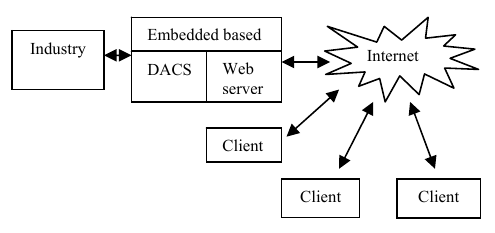
\includegraphics[scale=0.8]{embedded_web_server.png} 
    \label{fig:DJp1}
    \end{subfigure}
%    \begin{subfigure}{0.5\textwidth}
%    \includegraphics[width=1.0\linewidth, height=5cm]{images/DJ_profile2.png}
%    \label{fig:DJp2}
%    \end{subfigure}
 
 \caption{Embedded Web-Server Architecture}
\label{fig6}
\end{figure}



\subsection{Reason for choosing RTOS}

The RTOS manages all the required tasks in parallel and in small amounts of time. Web based management
user interfaces using embedded web server have many advantages: ubiquity, user-friendly, low-development cost
and high maintainability. Embedded web server is employed based on the  requirement such as low resource usage, high
reliability, security, portability and controllability for which general web server technologies are unsuitable.


\subsection{Software Design of the system}
Unlike Linux, RTLinux provides hard real-time capability. It has a hybrid kernel architecture with a small real-time
kernel coexists with the Linux kernel running as the lowest priority task. This combination allows RTLinux to
provide highly optimized, time-shared services in parallel with the real-time, predictable, and low-latency execution.
Besides this unique feature, RTLinux is freely available to the public. 
 

  \begin{figure}[H]
 
    \begin{subfigure}{\textwidth}
    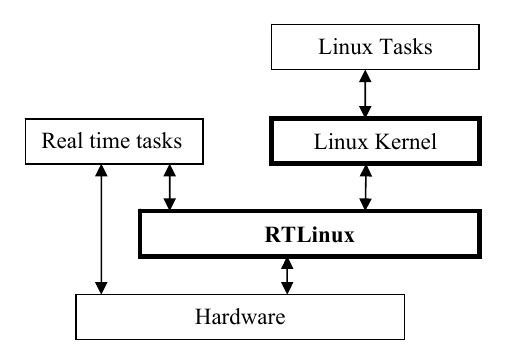
\includegraphics[scale=0.8]{rtlinux.png} 
    \label{fig:DJp1}
    \end{subfigure}
%    \begin{subfigure}{0.5\textwidth}
%    \includegraphics[width=1.0\linewidth, height=5cm]{images/DJ_profile2.png}
%    \label{fig:DJp2}
%    \end{subfigure}
 
 \caption{Run-time model of RT linux}
\label{fig6}
\end{figure}


\subsection{Components of a RTOS}
A real-time operating system includes multiple components as follows:
\begin{itemize}
    \item \textbf{The scheduler:} This is the main RTOS element that determines the order of execution of tasks or threads usually based on a priority scheme, and either in a run to completion or round robin fashion. Some RTOS may try to load balance thread across processors but most require developers to assign process affinity to cores to optimize real-time application resource usage.

\item \textbf{Symmetric Multiprocessing (SMP):} An RTOS has the ability to handle and separate multiple tasks or threads so that they can be run on multiple cores to allow for parallel processing of code (i.e. multitasking).

\item  \textbf{Function library:} Is a standard interface that can contain an application program interface (API) to call routines within it, this is the interface that connects that application code and the kernel. Application code entities direct requests to the kernel via the function library to prompt the application to give the desired programmatic behavior.

\item  \textbf{Fast dispatch latency/context switch time:} Dispatch latency represents the time from when the operating system identifies that a task has finished and until a ready to run thread is started or when an event is triggered that causes a higher priority tasks to preempt a currently running task. The context switch is the time it takes for the scheduled to switch from one running thread to another thread, this involved saving off the context of the current task and replacing it with the context of the new thread to run.In an RTOS, the switching time should remain deterministic and minimal.

\item  \textbf{User-defined data objects and classes:} An RTOS relies on programming languages with data structures that are organized based on their type of operation. The user defines object sets through a specified programming language like C++ that the RTOS will use in to control the specified application.

\item  \textbf{Memory Management:} Memory management is required to allocate memory for every program to be run or object to be referenced in memory. In an RTOS this is important, since unlike General Purpose OSes like Windows it can’t afford to have memory paged in or out since it leads to non-deterministic behavior.

\end{itemize}
























\subsection{Feasibility}
An SOC (System On Chip) shall be employed to achieve this desired goal.  To meet the above requirements a combination of software and hardware needs to be implemented. Thus, an embedded system shall be designed in a RTlinux specifically petalinux in an embedded Web-server architecture.




\newpage
\section{Phase 3: Designing Mechanical fixture}
Mechanical fixture to hold all the eight sensors needs to be designed. The design shall encompass both the technical and user convenience aspects.
        \begin{itemize}
            \item \textbf{ Technical aspect:} 
            
            This stand-alone system shall be custom designed considering the thermal aspects inculcating   hardware awareness and communicates with its peripherals  using different serial communication protocols like UART, SPI or I2C. 
            
            \item \textbf{ Lotus shaped Fixture:}
            
            During design, not only technical part but ease of use for the user also needs to be taken into account. A lotus shaped mechanical fixture shall be designed for housing the eight accelerometers  
        \end{itemize}



\newpage
\section{Phase 4: A Desktop application}
A Desktop application to access and analyse data from a local server is also planned. Taking into consideration that the networking issues should not effect the data logging, a local server is also planned. In case of any networking issues, the user can shift to desktop application and log the data into the local server. This desktop application shall  be built with these three-fold features:
\begin{enumerate}
    \item \textbf{Acquire:} The multiple weeks 
    \item \textbf{Retrieve:} This software shall be able to retrieve data from the local server for the purpose of verification for the user
    \item \textbf{Analyze:} The Post-acquisition analysis that includes myriad calculations shall be performed for generating a validatory report.
    \item \textbf{Represent:}Representation of data is one of the crucial steps for obtaining insights in projects like these. The software developed would portray the data as per the guidelines of the user to obtain meaningful conclusions from the data.
\end{enumerate}












\newpage

 \section{Validation}
 \textcolor{red}{Re-work necessary}
In short, DAQ can be validated by the user by acquiring the data from all the Eight acccelerometer sensors. The data obtained in their desired format validates the project.


\newpage
\section{Facilities, equipment and other Resources required}

\subsection{Data Infrastructure and Software needs}
\begin{itemize}
    \item Access to  Cloud intranet if available
    \item Vivado design suite for programming Xilinx SOC FPGA
    \item Few verilog  Private IP Cores.
\end{itemize}


\subsection{Deliverables}

\begin{itemize}
    \item A Complete standalone DAQ system with mechanical fixtures consisting of:
     \begin{enumerate}
         \item IOT enabled SOC 
         \item Mechanical fixtures/jigs for housing accelerometers
         \item An independent power supply or an in-house with three independent channels with less than 5 mV ripple V$_{rms}$.
     \end{enumerate}
    \item USB type C cable
    \item Software for post-analysis and graphical representation
    \item Two USB extenders 
    \item Ethernet switch
    \item Networking cables
    \item A local server, in case a cloud intranet is unavailable
 \end{itemize}

\section{Project Budget}
 \subsection{Cost-cutting}
Many other alternative plans have been proposed. This route and budget is proposed after a series of discussions with RCI incharges regarding their technical requirement for a turn-key solution.

\subsection{Intellectual Merit}
We offer a high-end, high-tech simulation, automation and precision  manufacturing solutions. Our group comprises of accomplished professionals from a variety of backgrounds, including electrical, software, mechanical,  underground instrumentation and measurement. We offer solutions to improve the quality, durability, and reliability of the final products, processes or tasks. 

\newpage

\subsection{Human Resources}
A Doctorate holding professional shall be made in-charge for this entire project. He shall be overlooking the entire project and guides the engineers to implement it successfully. He shall be on-looking three other projects, which happens to be 20,000. 
\begin{center}
\begin{tabular}{||p{2 cm} ||p{3 cm}||p{1.5 cm}|| p{1.5 cm}|| p{2 cm}||p{3 cm}|| }
\arrayrulecolor{Azzurro}
\hline
\hline

{\bfseries Human Resource } & {\bfseries Role} & {\bfseries personnel}&{\bfseries Man Month}& {\bfseries Duration (months)} & {\bfseries Cost INR} \\
\hline
\hline
 Doctorate holding Professional  & In-charge and overlooks the entire project &1 & 20,000 & 8 months & 8 months$\times$ 20,000=1,60,000\\
\hline
\hline
VHDL (verilog) Programmer& Design and optimization of the hardware, one looks after electronics and the other looks after communication  &1 & 45,000 & 8 months & 8 months $\times$ 45,000=3,60,000\\
\hline
\hline
Electrical engineer &Programming for the interfacing, low level interfacing using C and high level integration with python  &1 & 45,000 & 8 months & 8 months $\times$ 45,000=3,60,00\\
\hline
\hline
& & & Total & & 8,80,000
\end{tabular}
\end{center}

\newpage
\subsection{Human resource sub division of work table for DAQ system and its associated software development}

\begin{center}
\begin{tabular}{||p{3 cm} ||p{4 cm}|| p{6 cm}|| |p{2 cm}|| }
\arrayrulecolor{Azzurro}
\hline
\hline

{\bfseries Phase/Item name } & {\bfseries Operation}& {\bfseries Description} & {\bfseries Human resource no.} \\
\hline
\hline
Design phase and Hardware finalization& Proteus as hardware simulation environment and Keil as
software design environment &  Aspects like required  processing speed, Memory, Storage, Energy consumption considered. GPIO, Timers, serial ports and Analog to digital converters shall also be made available. communication protocols like UART, SPI shall be established &1\\
\hline
\hline
Hardware procurement & &Online ordering and manual procurement of components & 1 \\
\hline
\hline
PCB designing & utilization Proteus Schematic Capture and PCB Layout modules  & Licensing of Proteus Enterprise Edition costed us&2\\ 
\hline 
\hline
PCB Manufacturing for prototyping & Shall be procured from a local vendor which includes both manufacturing and population charges & This shall be utilized to get approval from the user&1 \\
\hline 
\hline
software integration with hardware &Keil as
software design environment & This involves coding for three modes of operation discussed above  & 2\\
\hline
\hline
&  &Total number of Human resources required & 2 numbers
 
 \end{tabular}
\end{center}











\newpage

\subsection{Costs incurred for Product Development}

\definecolor{Gray}{gray}{0.9}
\definecolor{LightCyan}{rgb}{0.88,1,1}
\definecolor{orange}{rgb}{1,0.86,0.5}

\begin{table}[ht]
%\color{white}
\setlength{\extrarowheight}{15pt}
\begin{tabular}{||p{3 cm} ||p{4 cm}|| p{5 cm}|| p{2 cm}|| }
\hline
\hline
\rowcolor{orange}
\hline
\hline


{\bfseries Phase/Item name } & {\bfseries Operation}& {\bfseries Description} & {\bfseries Cost INR} \\

\arrayrulecolor{white}

\rowcolor{Gray}
\hline
\hline
Virtex SOC &Field Programmable Gate array with SOC capability&Than a multiple chip BOM this tends to be cheaper (from mouser) &1,54,582.82\\
\rowcolor{Gray}
\hline
\hline
Casing& For protection of the board& &6,500 \\
\rowcolor{Gray}
\hline
\hline
Accessory cards required &&  & 10,000  \\
\hline
\hline

\rowcolor{Gray}

Mechanical Fixtures& & & 15,000\\

\rowcolor{Gray}
\hline
\hline
Vivado Design suite&IDE and synthesis tools&Includes monthly EMI paid+few Private IPs&16,000 \\

\hline
\hline


& Total & & XXXX
\end{tabular}
\end{table}



\newpage
\subsection{Resources required}
\begin{center}
\begin{tabular}{||p{3 cm} ||p{4 cm}|| p{6 cm}|| c|| }
\arrayrulecolor{Azzurro}
\hline
\hline
{\bfseries S.No} & {\bfseries Item Name}& {\bfseries Item Description} & {\bfseries Cost (Rs)} \\
\hline
\hline
Nine extender's for accelerometer &straight cable D-pin connectors & Required for aesthetic connections & 1000\\
\hline
\hline
Two mini USB extenders & Male to female mini USB connectors& Extend the communication from the embedded system to the computer, 3000 $\times$2 & 6000\\
\hline
\hline
Windows 7/8 software & &   & 8000\\
\hline
\hline
Ethernet switch & Required for networking & &1000\\
\hline
\hline
Networking Cables & 2 to 3 cables & Required for networking &500\\
\hline
\hline
& Total & & 16,500
 
 \end{tabular}
\end{center}





\subsection{Total Budget}
\begin{center}
\begin{tabular}{||c ||p{6 cm}|| p{3 cm}|| c|| }
\arrayrulecolor{Azzurro}
\hline
\hline
{\bfseries S.No} & {\bfseries Budget}&  {\bfseries Cost INR} \\
\hline
\hline

1& High end PC& 1,04,800\\
\hline
\hline
2& Costs incurred for Product Development & 60,000\\
\hline
\hline
3&Resources required &16,500\\
\hline
\hline
4&Human Resources & 8,80,000\\
\hline
\hline
& Total & Dont know
\end{tabular}
\end{center}





\section{Conclusion}
With the rapid development of the field of industrial process control and the wide range of applications of network, intelligence, digital distributed control System, we generally design a higher data accuracy and
reliability  control system. This embedded ARM system can adapt to the strict requirements of the data acquisition and control system such as the function, reliability, cost, size, power consumption, and remote access
and so on. This system operated by DACS mode to acquire the signals and control the devices remotely. Embedded web server mode is used to share the data with clients in online. Both modes are efficiently carried out by real time multi tasking operating system (RTLinux). 














\newpage











\end{document}